\chapter{Волновые свойства частиц}

\section{Волна де Бройля}

Развитие квантовой теории началось с того, что у света наряду с волновыми свойствами, характеризуемыми длиной волны $\lambda$ и частотой $\omega$, были обнаружены также и корпускулярные. Значения для энергии $E$ и импульса $\vp$ кванта света были установлены Альбертом Эйнштейном в 1905~г.

\begin{equation}
\label{eq:1_1_1}
\begin{gathered}
E = \hbar \omega \\ 
\vp = \hbar \vec{k}
\end{gathered}
\end{equation}

Здесь $\hbar = 1{,}05 \cdot 10^{-27}$ эрг·с -- постоянная Планка, была впервые введена Максом Планком в 1900~г. для объяснения спекторв испускания нагретых тел; $\vec{k}$ -- волновой вектор. В соотношениях \eqref{eq:1_1_1} корпускулярные ($E$ и $\vp$) и волновые ($\omega$ и $\vec{k}$) свойства света связаны постоянной Планка.

Анализируя эти соотношения, французский физик Луи Виктор де Бройль в 1923~г. выдвинул гипотезу о возможности их обобщения на всех массивные частицы (идея материальных волн или волн вещества). Иными словами, де Бройль предположил, что дуализм <<волна-частица>> должен быть свойственен не только свету, но и электронам и любым другим частицам (<<дуализм>> означает двойственность).

Соответствующая частица и волновое число определяются при этом соотношениями, подобными эйнштейновским \eqref{eq:1_1_1}, т.е. длина де-бройлевской волны движущихся частиц будет равна

\begin{equation}
\label{eq:1_1_2}
\lambda = \frac{2\pi}{k} = \frac{2\pi \hbar}{p} = \frac{h}{mv}
\end{equation}

Известно, что распространение фотонов (квантов света), т.е. распространение света с частотой $\omega$ и волновым вектором $\vec{k}$, описывается плоской волной

\begin{equation}
\label{eq:1_1_3}
\Psi (\vr, t) = A e^{i(\vec{k}\vr - \omega t)}
\end{equation}

В выражении \eqref{eq:1_1_3} заменим $\omega$ на $\vec{k}$, используя формулы \eqref{eq:1_1_1}

\begin{equation}
\label{eq:1_1_4}
\boxed{\Psi(\vr,t) = A e^{\frac{i}{\hbar}(\vp\vr - Et)}}
\end{equation}

Волновой функцией \eqref{eq:1_1_4} фотона является световая волна; движущейся частице с энергией $E$ и импульсом $\vp$, согласно гипотезе де Бройля, соответствует волновая функция такого же вида \eqref{eq:1_1_4} или \underline{волны де Бройля}.

\begin{sloppypar}
  \section{Волновой пакет. Фазовая и групповая скорость волн, соответствующих свободной частице}
\end{sloppypar}

Пусть свободная частица с энергией $E$ и импульсом $\vp$ движется вдоль оси $x$, т.е. $\vp~ \|~ \vec{x}$. Сопоставим движущейся частице волну де Бройля

\begin{equation}
\label{eq:1_2_1}
\Psi(x,t) = A e^{\frac{i}{\hbar}(px - Et)}
\end{equation}%
%
В ней поверхность востоянной фазы $\alpha = kx - \omega t$ перемещается с фазовой скоростью

\begin{equation}
\label{eq:1_2_2}
v_{\text{ф}} = \frac{dx}{dt} = \frac{w}{k} = \frac{E}{p}
\end{equation}%
%
В нерелятивистском случае $E = p^2/{2m}$, следовательно
$$
v_{\text{ф}} = \frac{p}{2m} = \frac{v}{2}
$$
т.е. фазовая скорость не совпадает с классической скоростью частицы $v$. Более того, в релятивистском случае $p = Ev/c^2$, или
$$
v_{\text{ф}} = \frac{E}{p} = \frac{c^2}{v} > c
$$
Эти результаты говорят о том, что плоская монохроматическая волна \underline{принципиально не может описывать свободную частицу}.

Чтобы выйти из этого положения и в то же время сохранить за частицами их волновые свойства, нашедшие блестящие экспериментальные подтверждения\footnote{Опыты Клинтона Джозефа Девисона и Лестера Халберта Джермера в 1927~г. по дифракции электронов, а также независимые опыты Джорджа Паджета Томсона в том же году.}, необходимо, не отказываясь от волны де Бройля, выработать более глубокий подход к описанию свободной частицы. На первых же порах развития квантовой механики стали сопоставлять частицам не отдельные монохроматические волны, а набор волн, обладающий близкими частотами. Такой подход подсказывался ещё и тем обстоятельством, что наблюдаемые на опыте дифракционные линии электронных волн всегда характеризовались определённой шириной, т.е. дифрагировали как бы не одна, а ряд волн, очень близких друг к другу по частоте.

Кроме того, если использовать не отдельную монохроматическую волну, а набор волн с близкими частотами, то с их помощью всегда можно построить такой волновой пакет, результирующая амплитуда которого окажется заметно отличной от нуля лишь в некоторой небольшой области пространства, котору. можно связать с местоположением частицы. Заметим, что плоская монохроматическая волна не локализована в пространстве, и потому она не может быть сопоставлена локализованному объекту, к каковому относится массивная частица.

Исходя из приведённых выше соображений, построим для описания движения частицы волновой пакет из непрерывной совокупности монохроматических плоских волн \eqref{eq:1_1_3}

\begin{equation}
\label{eq:1_2_3}
\Psi(x,t) = \int^{k_0 + \Delta k}_{k_0 - \Delta k} A(k)e^{i(\vec{k}\vr - \omega (k) t)} dk, \; \Delta k\ll k_0
\end{equation}

Здесь $k_0$ -- волновое число центра пакета, около которого сосредоточены волновые числа волн, образующих волновой пакет. Считаем, что $\Delta k \ll k_0$.

В отличие от \eqref{eq:1_1_3}, волновой пакет -- это группа волн с различными (хотя и близкими) величинами волнового числа $k$, а значит, и частоты

\begin{equation}
\label{eq:1_2_4}
\omega (k) = \omega (k_0) + \left. \left ( \frac{d \omega}{dk} \right ) \right |_{k_0} (k-k_0) + \ldots \approx \omega_o +  \left. \left ( \frac{d \omega}{dk} \right ) \right |_{k_0} (k-k_0)
\end{equation}%
%
С помощью \eqref{eq:1_2_4} и \eqref{eq:1_2_3} найдём
\begin{equation}
\label{eq:1_2_5}
\psi(x,t) \approx e^{i(k_0 x - \omega_0 t) }\int^{k_0 + \Delta k}_{k_0 - \Delta k} dk A(k)e^{i(k - k_0) \left [ x - \left . \left ( \frac{d\omega}{dk} \right ) \right |_{k_0} t \right ]}
\end{equation}%
%
Т.е. волновая функция пакета есть плоская волна, отвечающая центру пакета $(k_0, \omega_0)$, амплитуда которой зависит от координаты и времени лишь через комбинацию
$$
x - \left . \left ( \frac{d\omega}{dk} \right ) \right |_{k_0} t
$$
Поэтому для всех точек $x$ и моментов времени $t$, связанных условием
\begin{equation}
\label{eq:1_2_6}
x - \left . \left ( \frac{d\omega}{dk} \right ) \right |_{k_0} t = \const
\end{equation}
амплитуда имеет одинаковое значение: волновой пакет движется как одно целое с групповой скоростью
\begin{equation}
\label{eq:1_2_7}
v_{\text{гр}} = \frac{dx}{dt} = \left . \left ( \frac{d\omega}{dk} \right ) \right |_{k_0} = \left . \left ( \frac{dE}{dp} \right ) \right |_{p_0}
\end{equation}%
%
как в нерелятивистском случае, когда $E = p^2/{2m}$
$$
v_{\text{гр}} = \frac{p_0}{m} = v
$$
так и в релятивистском случае, когда $E = \sqrt{p^2c^2 + m^2c^4}$
$$
v_{\text{гр}} = \frac{c^2 2p}{2E} = \frac{c^2 \frac{E}{c^2}v}{E} = v
$$

\underline{Таким образом, групповая скорость перемещения волнового пакета как целого точно совпадает со скоростью $v$ движения соответствующей ему частицы.}

Взяв $k - k_0 = \xi$ в качестве новой переменной интегрирования и считая $A(k)$ слабо меняющейся на ширине пакета функцией $k$, найдём, что $\Psi(x,t)$ может юыть представлена с учётом \eqref{eq:1_2_5} и \eqref{eq:1_2_7} в виде%
%
$$
\Psi(x,t) \approx A(k_0) e^{i(k_0 x - \omega_0 t) }\int^{+ \Delta k}_{ - \Delta k} e^{i(x - v_{\text{гр}}t)\xi} d\xi
$$%
%
Выполняя интегрирование по $\xi$, найдём
\begin{equation}
\label{eq:1_2_8}
\Psi(x,t) =
  \underbrace{
    2 A(k_0) \frac{\sin [(x - v_{\text{гр}}t)\Delta k]}{x - v_{\text{гр}}t}
  }_{B(x - v_{\text{гр}}t)}
  e^{i(k_0 x - \omega_0 t)} = B(x - v_{\text{гр}}t) e^{i(k_0 x - \omega_0 t)}
\end{equation}%
%
Т.к. под знаком синуса стоит малая величина $\Delta k$ ($\Delta k \ll k_0$), то \underline{амплитуда волнового пакета} $B(x - v_{\text{гр}}t)$ будет медленно меняющейся функцией координаты и времени, поэтому её можно рассматривать как огибающую почти монохроматической волны, а $(k_0 x - \omega_0 t)$ -- как её фазу. Причём эта огибающая, как было показано выше, перемещается в пространстве с групповой скоростью $v_{\text{гр}}$.

Определим координату $x$, где амплитуда $B(x - v_{\text{гр}}t)$ имеет максимум. Очевидно, искомый максимум будет находиться в точке
$$x = v_{\text{гр}}t$$
т.е. максимум амплитуды отвечает выбору $\const = 0$ в \eqref{eq:1_2_6}. График функции $\Re\brc{\Psi(x, 0)}$ представлен на \autoref{fig:1_1}.

\begin{figure}[h]
\centering
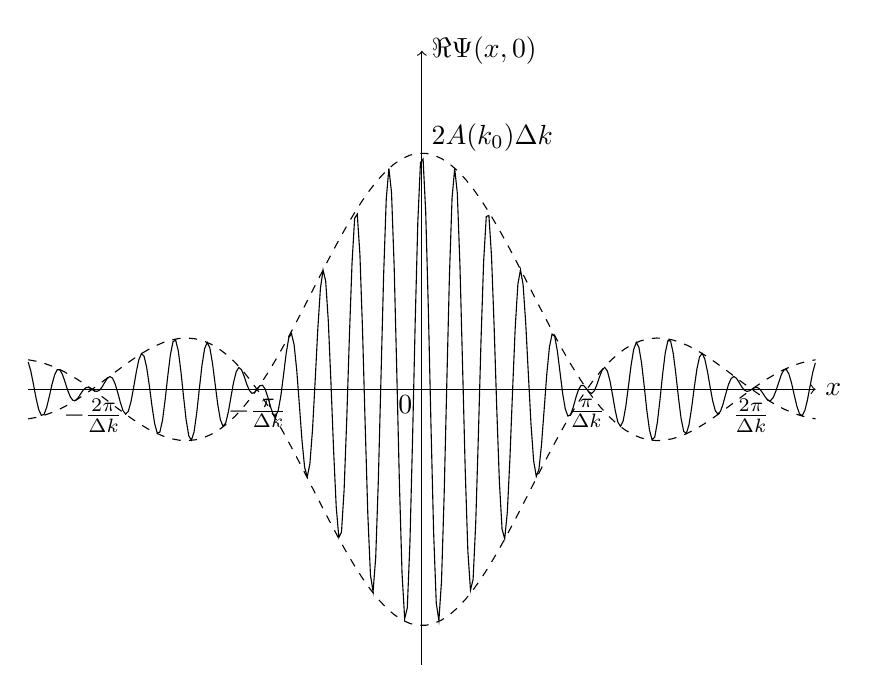
\begin{tikzpicture}[domain=-5:5]
  \draw[->] (-5,0) -- (5,0) node[right] {$x$};
  \draw[->] (0,-3.5) -- (0,4.3) node [right] {$\Re\brc{\Psi(x, 0)}$};
	\draw [dashed, domain=-5:5, samples=100] plot (\x, {2*sin(1.5*\x r) / \x});
  \draw [dashed, domain=-5:5, samples=100] plot (\x, {-2*sin(1.5*\x r) / \x});
  \draw [domain=-5:5, samples=300] plot (\x, {2*sin(1.5*\x r)*cos(15*\x r) / \x});
  \node [left] at (0, -0.2) {$0$};
  \node [below] at (2.09, 0) {$\frac{\pi}{\Delta k}$};
  \node [below] at (-2.09, 0) {$-\frac{\pi}{\Delta k}$};
  \node [below] at (4.18, 0) {$\frac{2\pi}{\Delta k}$};
  \node [below] at (-4.18, 0) {$-\frac{2\pi}{\Delta k}$};
  \node [right] at (0, 3.2) {$2A(k_0) \Delta k$};
\end{tikzpicture}
\caption{Форма волнового пакета при $t=0$.} \label{fig:1_1}
\end{figure}


При $t = 0$ своего наибольшего значения $B(0) = 2A \delta k$ амплитуда достигает в точке $x = 0$. Во всех остальных точках, соответствующих локальным максимумам, амплитуда будет существенно меньше. Таким образом, волновой пакет можно считать локализованным в области абсолютного максимума, т.е. в области шириной $\Delta x = 2\pi / \Delta k$ (см. график). Т.к. $k_0 \gg \Delta k$, то для длины волны имеем
$$
\lambda = \frac{2 \pi}{k_0} \ll \frac{2 \pi}{\Delta k} = \Delta x
$$%
%
т.е. длина де-бройлевской волны многократно укладывается на ширине пакета.

В силу модельного характера описания волнового пакета \eqref{eq:1_2_3}, т.е. принятия модельных соображений относительно зависимостей $\omega(k)$ и $A(k)$, запишем соотношение между разбросом $\Delta k$ волновых чисел и шириной области пространственной локализации пакета $\Delta x$ по порядку величины:
\begin{equation}
\label{eq:1_2_9}
\Delta x \cdot \Delta k \approx 1 ~\text{\footnotemark}
\end{equation}

\footnotetext{Это соотношение справедливо для описания волнового процесса произвольной природы. Например, тот, кто знаком с радиофизикой, знает, что для посылки короткого радиосигнала (малое $\Delta x$) требуется широкий набор волн различной длины. Поэтому такой сигнал будет принят приёмниками, настроенными на различные волны. Напротив, если мы желаем, чтобы его принимали приёмники, настроенные лишь определённым образом, то необходимо посылать достаточно длинные, почти монохроматические сигналы.}

По уравнению \eqref{eq:1_1_1} для группы волн де Бройля получим из \eqref{eq:1_2_9} соотношение
\begin{equation}
\label{eq:1_2_10}
\boxed{\Delta p \cdot \Delta x \approx \hbar}
\end{equation}

Это соотношение было впервые установлено Вернером Карлом Гайзенбергом в 1927~г. Его принято называть \underline{соотношением неопределённостей Гайзенберга}: <<чем точнее определено положение, тем менее точно известен импульс, и наоборот>>. Таким образом, не существует состояния, в котором частица одновременно имела бы определённые значения координаты и импульса. Следовательно, теряет смысл понятие траектории микрочастицы, подразумевающее определение в каждый момент времени значений координаты и скорости (или импульса). Соотношение неопределённостей есть следствие и математическое выражение корпускулярно-волнового дуализма природы материи. Мы не можем в любой момент времени $t$ приписать частицы определённое положение $\vr$. Вместо этого мы вводим волновую функцию частицы $\Psi(\vr, t)$.


\begin{sloppypar}
  \section{Уравнение Шрёдингера. Оператор Гамильтона. Общее решение уравнения Шрёдингера в случае, когда гамильтониан не зависит от времени. Стационарное уравнение Шрёдингера}
\end{sloppypar}

Гипотеза де Бройля, согласно которой каждой частице сопоставляется волна, вскоре была развита, и на её основе была создана новая механика. Действительно, если есть волны, то должно быть и волновое уравнение. Поэтому надо было найти такое динамическое уравнение, которое описывало бы распространение волн де Бройля в пространстве и времени, т.е. эволюцию волновой функции $\Psi(\vr, t)$. Ясно, что это уравнение не может быть выведено из предыдущих теорий, наоборот, их результаты должны получаться из решений искомого уравнения как предельные случаи. Эрвин Шрёдингер в 1926~г. фактически постулировал волновое уравнение, следуя оптико-механической аналогии Гамильтона и идее волн де Бройля
\begin{equation}
\label{eq:1_3_1}
\boxed{
  i \hbar \pd{\Psi(\vr,t)}{t} =
    \brcr{-\frac{\hbar^2}{2m}\vec{\nabla}^2 + U(\vr,t)} \Psi(\vr,t)
} 
\end{equation}%
%
позже названное временным (нестационарным) уравнением Шрёдингера (УШ). Выражение в фигурных скобках интерпретируется как оператор полной нерелятивистской энергии, или оператор Гамильтона (гамильтониан):
$$
\op{H} = \frac{\op{\vp}^2}{2m} + U(\vr,t)
$$
\begin{equation}
\label{eq:1_3_2}
i \hbar \pd{\Psi(\vr,t)}{t} = \op{H} \Psi(\vr,t)
\end{equation}

Пусть оператор Гамильтона на зависит явно от времени, т.е.
$$\pd{\op{H}}{t} = \pd{U}{t} = 0$$
В классической механике это означало бы, что функция Гамильтона постоянна во времени и равна полной энергии системы (интеграл движения). В квантовой механике в этом случае явная зависимлсть от времени может быть только у волновой функции (ВФ) $\Psi(\vr,t)$, причём можно искать решение \eqref{eq:1_3_2} методом разделения пространственных и временных переменных:%
%
\begin{equation}
\label{eq:1_3_3}
\Psi(\vr,t) = \psi(\vr) \cdot \phi (t)
\end{equation}%
%
Тогда, поставляя такую функцию \eqref{eq:1_3_3} в УШ \eqref{eq:1_3_2}, получим
$$
i \hbar \psi(\vr) \pd{}{t} \phi (t) = \phi (t) \op{H} \psi(\vr)
$$%
%
Поделив обе части на ВФ \eqref{eq:1_3_3}, придём к соотношению
\begin{equation}
\label{eq:1_3_4}
i \hbar \frac{\partial \phi / \partial t}{\phi(t)} = \frac{\op{H} \psi(\vr)}{\psi(\vr)}
\end{equation}
Левая часто полученного соотношения зависит только от времени $t$, а правая -- только от пространственных переменных $\vr$. Поскольку время и пространственные переменные независимы, то для произвольных $t$ и $\vr$ равенство возникает лишь в случае, когда обе части по отдельности равны одной и той же постоянной величине $E$. Как следует из \eqref{eq:1_3_4}, в этом случае мы приходим к двух уравнениям, определяющим отдельно функции $\phi(t)$ и $\phi(\vr)$:
\begin{equation}
\label{eq:1_3_5}
i \hbar \pd{}{t} \phi(t) = E \phi(t)
\end{equation}

\begin{equation}
\label{eq:1_3_6}
\boxed{\op{H} \psi(\vr) \equiv \left\{ -\frac{\hbar^2}{2m} \vec{\nabla}^2 + U(\vr) \right\}\psi(\vr) = E\psi(\vr)}
\end{equation}

Первое из этих уравнений имеет решение
$$
\phi(t)=C e^{-iEt/\hbar}
$$
где $C$ -- постоянная интегрирования, определяемая из начальных условий $C = \phi(0)$. Координатная часть $\psi(\vr)$ ВФ \eqref{eq:1_3_3} удовлетворяет \underline{стационарному уравнению Шрёдингера}. Входящая в него постоянная разделения переменных $E$ имеет размерность энергии. С точки зрения уравнений математической физики, стационарное УШ есть частный случай задачи Штурма-Лиувилля на собственные значения гамильтониана и отвечающие им собственные функции, т.е. собственные пары $\{E_k, \psi_k(\vr)\}$. Таким образом, константа разделения $E$ является собственным значением гамильтониана, а по физическому смыслу соответствует дискретным значениям полной энергии системы. Термин <<стационарные состояния>> означает состояния с определённой энергией.

\begin{sloppypar}
  \section{Статистическая интерпретация волновой функции. Стационарные состояния}
\end{sloppypar}

В отличие от уравнения Ньютона, из которого находится наблюдаемая траектория $\vr(t)$ материальной точки, из уравнения Шрёдингера находят в общем случае комплексную, т.е. ненаблюдаемую, волновую функцию $\Psi(\vr, t)$ квантовой системы. Тем не менее, как будет показано ниже, с её помощью можно вычислить значения всех измеримых величин. Сразу же после открытия УШ, Макс Борн (1926~г.) дал статистическую интерпретацию ВФ $\Psi(\vr, t)$.

Величина
\begin{equation}
\label{eq:1_4_1}
dP = \Psi^*(\vr,t) \Psi(\vr,t) dv \equiv \abs{\Psi(\vr,t)}^2dv
\end{equation}%
%
представляет вероятность нахождения частицы в момент времени $t$ в элементе объёма $dv$ в окрестности точки $\vr$. Интенсивность волны
\begin{equation}
\label{eq:1_4_2}
\abs{\Psi(\vr,t)}^2 = \frac{dP}{dv} = \rho(\vr,t)
\end{equation}%
%
интерпретируется как плотность вероятности нахождения частицы в точке $\vr$ в момент времени $t$. Тогда ВФ $\Psi(\vr, t)$ -- амплитуда плотности вероятности, или просто \underline{амплитуда вероятности}. Если произвести интегрирование \eqref{eq:1_4_1} по всему бесконечному объёму, то мы получим вероятность достоверного события обнаружить частицы где-либо в пространстве, равную, очевидно, единице:
\begin{equation}
\label{eq:1_4_3}
\int \abs{\Psi(\vr,t)}^2 dv = 1
\end{equation}
Это условие называется \underline{условием нормировки}, а функция $\Psi$, удовлетворяющая этому условию, называется \underline{нормированной ВФ}. Для выполнимости такой нормировки, интеграл от $\abs{\Psi(\vr,t)}^2$ должен существовать (говорят, что функция $\Psi$ должна быть квадратично интегрируема). Соотношение \eqref{eq:1_4_3} выполняется для волнового пакета \eqref{eq:1_2_3}, но не выполняется для волны де Бройля \eqref{eq:1_1_4}: интеграл
$$
\int \abs{\Psi_{\vp}(\vr,t)}^2 dv = \abs{A}^2 \int dv
$$
не сходится. В дальнейшем мы дадим рациональную нормировку и для этого случая.

Нормировка имеет смысл лишь постольку, поскольку она сохраняется во времени, т.е. равенство \eqref{eq:1_4_3} должно иметь силу для всех моментов времени, т.е. вероятность найти частицу где-либо в пространстве не должна зависеть от времени, т.е.
$$
\pd{}{t} \int \rho(\vr,t) dv = 0
$$
\begin{excr}
Строго доказать, что $\Psi(\vr,t)$ удовлетворяет волновому уравнению \eqref{eq:1_3_1}
\end{excr}

Вероятностное толкование приводит к определённым требованиям для $\Psi(\vr,t)$: она должны быть (i) однозначной, (ii) конечной и \textit{(как правило, исключение: задача 4c из 1-го задания)} (iii) непрерывно дифференцируемой{\footnotemark}~функцией. Такими же свойствами должна обладать функция $\abs{\Psi(\vr,t)}^2$.

\footnotetext{т.е. $\Psi(\vr,t) \in C^1(\Omega)$ во всей области изменения её аргументов $\Omega$}

Если вернуться к анализу стационарного УШ \eqref{eq:1_3_6}, то на ВФ $\psi{\vr}$, как на решение задачи Штурма-Лиувилля, должны быть наложены условия i-iii с учётом её нормировки
\begin{equation}
\label{eq:1_4_4}
\norm{\psi} \equiv \int \abs{\psi(\vr)}^2 dv = 1
\end{equation}%
%
% TODO: в рукописи нет этого: Граничные условия: $\psi(\vr)|_{r \to \infty} = 0$
а также она должна удовлетворять заданным граничным условиям. Для временной части ВФ \eqref{eq:1_3_3} имеем: $\abs{\phi (t)}^2= \abs{C}^2$. Всегда можно положить $C = 1$, т.е. условия нормировки \eqref{eq:1_4_3} и \eqref{eq:1_4_4} определяются интегрированием по пространственным переменным. Таким образом, в случае, когда $\op{H}$ не зависит от времени, состояние с определённой и сохраняющейся во времени энергией $E$ (стационарное состояние) описывается волновой функцией
$$
\boxed{
  \Psi_E(\vr,t) = e^{-\frac{i}{\hbar}Et} \psi_E(\vr)
}
$$ где $\op{H} \psi_E(\vr) = E\psi_E(\vr)$. Волновая функция стационарного состояния зависит от времени, но эта зависимость входит только через фазу волны.
\\
\\

В заключении важно отметить, что статистическое описание характерно не для пучка частиц, а для каждой отдельной частицы. Например, в 1949~г. советские физики Л.~Биберман, Н.~Сушкин и В.~Фабрикант прямыми опытами для электронов доказали, что при малых интенсивностях пучка волновые свойства электронов не исчезают. Следовательно, $\Psi(\vr,t)$ следует рассматривать как синтез волновых, корпускулярных и статистических представлений о микрообъекте.